\chapter{基于攻击树的威胁建模}

\section{攻击树的构建}
打开sbid工具,点击左上角的[新协议]按钮,或在菜单栏中点击[文件>新协议],创建协议面板,在菜单栏中点击[模型>添加攻击树(Attack Tree)],打开攻击树面板。

\begin{figure}[h]
	\centering
	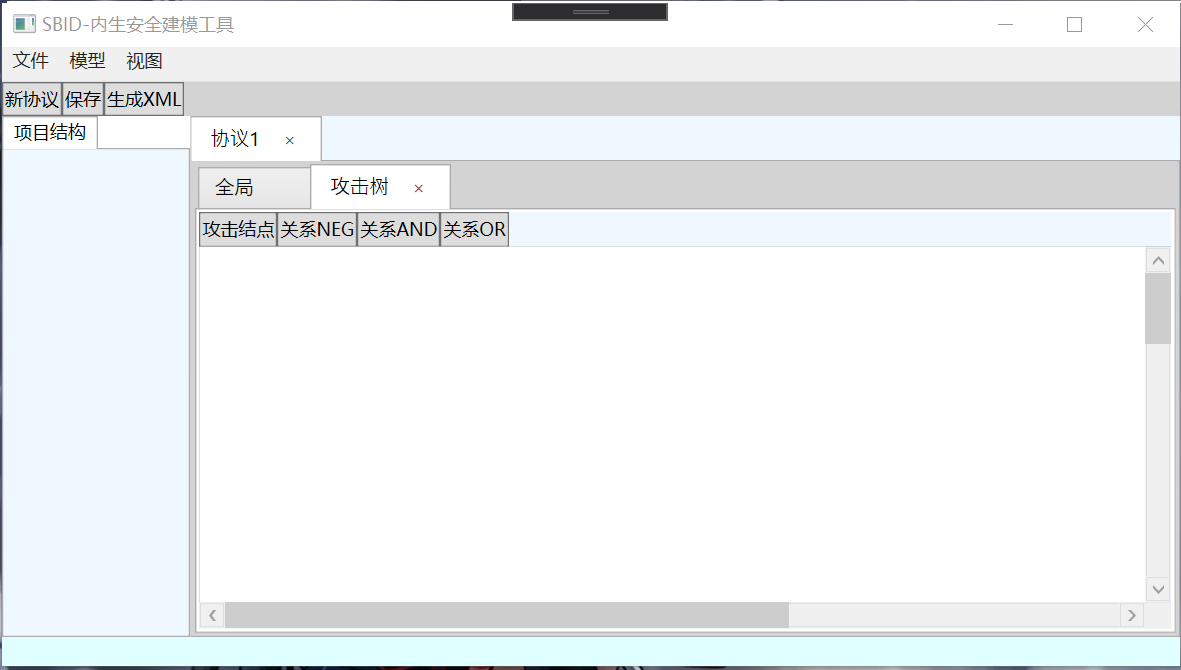
\includegraphics[width=12cm,height=6.75cm]{imgs/attack_tree_panel.png}
	\caption{创建攻击树面板}
	\label{attack_tree_panel}
\end{figure}

\par
点击小工具栏上的[攻击结点]、[关系NEG]、[关系AND]、[关系OR]按钮,即可创建相应结点。

\begin{figure}[h]
	\centering
	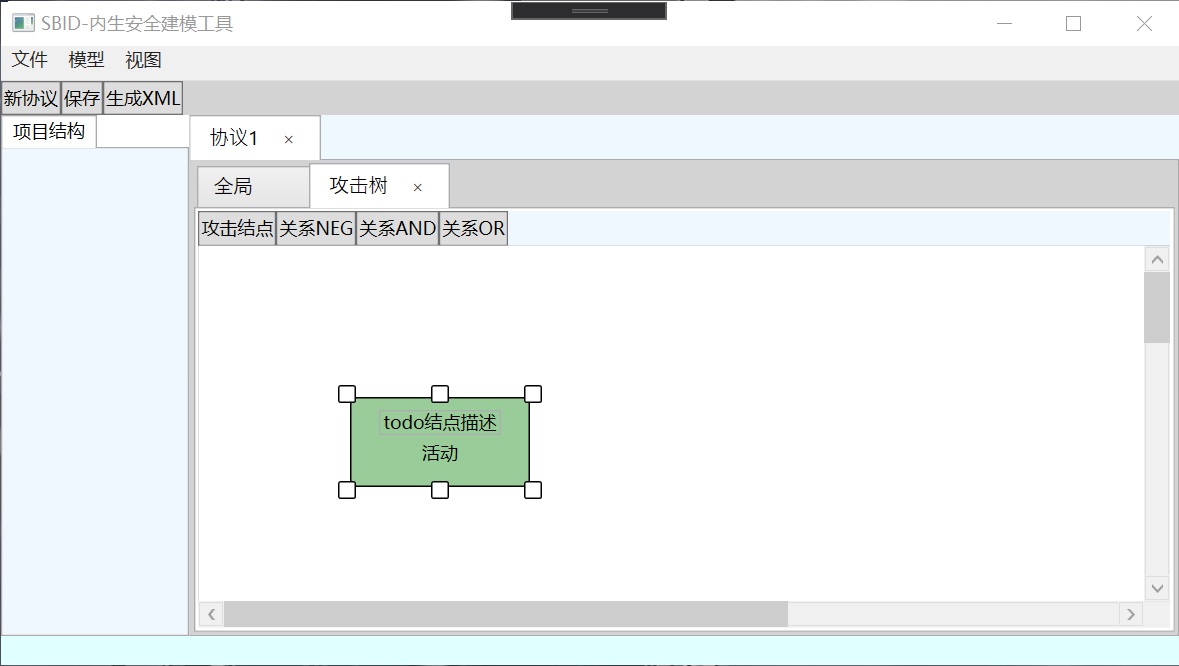
\includegraphics[width=12cm,height=6.75cm]{imgs/attack_tree_create_node.png}
	\caption{创建结点}
	\label{attack_tree_create_node}
\end{figure}

\par
攻击结点的输入框可以输入文字更改攻击结点描述。

\begin{figure}[h]
	\centering
	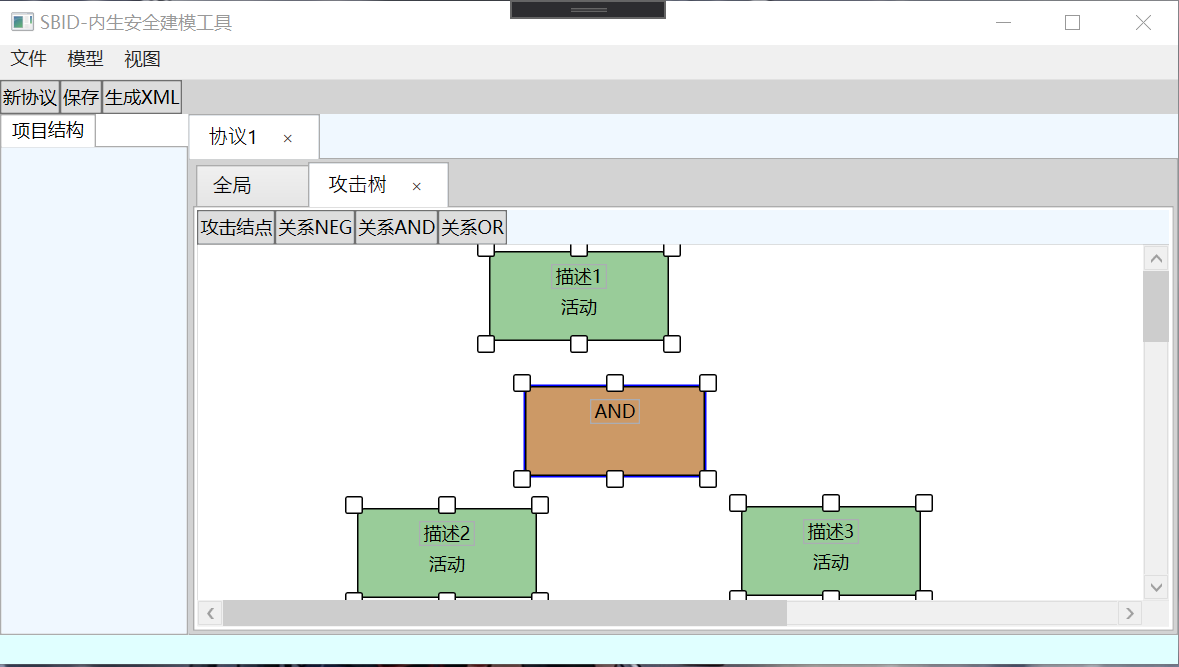
\includegraphics[width=12cm,height=6.75cm]{imgs/attack_tree_description.png}
	\caption{更改结点描述}
	\label{attack_tree_description}
\end{figure}

\par
创建结点后,可以点击结点周围的六个锚点并拖动鼠标连接其他结点,从而构造一棵攻击树。

\begin{figure}[h]
	\centering
	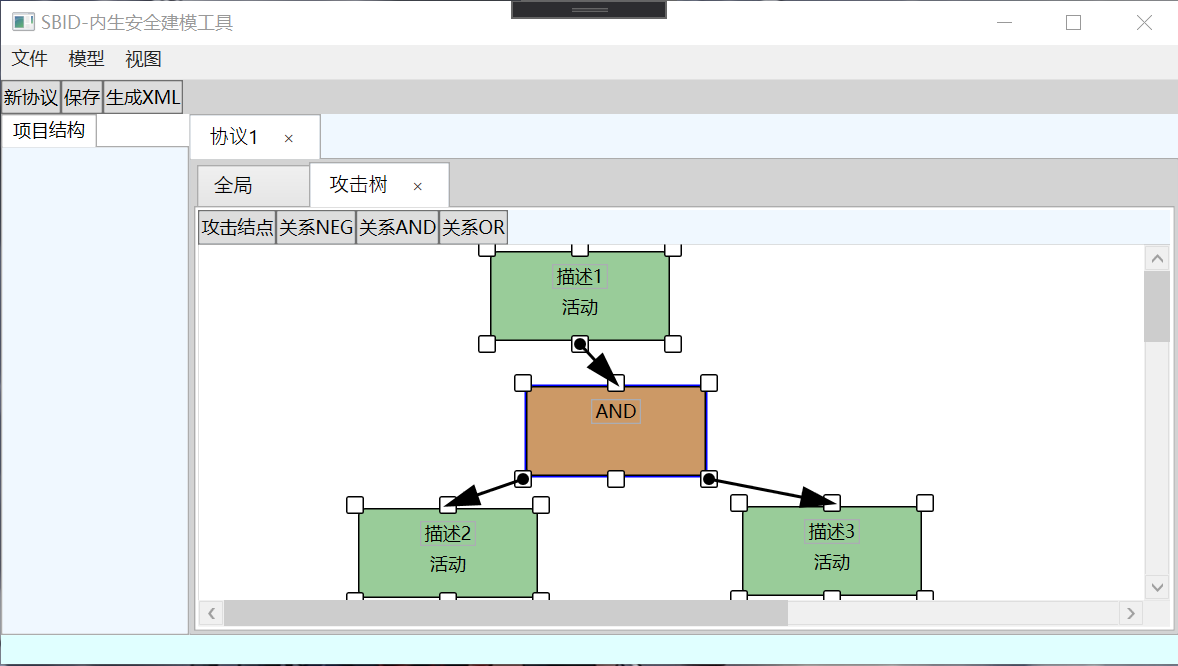
\includegraphics[width=12cm,height=6.75cm]{imgs/attack_tree_lines.png}
	\caption{连接结点}
	\label{attack_tree_lines}
\end{figure}

\section{威胁判定}
攻击树为我们提供了一种正式而条理清晰的方法来描述系统所面临的安全威胁和系统可能受到的多种攻击。
我们用树型结构来表示系统面临的攻击,其中根节点代表被攻击的目标,叶节点表示达成攻击目标的方法。

\par
攻击节点有两种状态:非活动的和活动的。
\par
非活动的攻击节点有确定的值,TRUE或者FALSE。
\par
活动的攻击节点的值由子节点计算得出。
\par
关系结点有三种,关系NEG结点、关系AND结点、关系OR结点,它们的计算逻辑为:
\par
NEG结点:仅有一个子节点,子节点为TRUE则该结点为FALSE,子结点为FALSE则该结点为TRUE。
\par
AND结点:若子节点中有至少一个结点为FALSE,则该结点为FALSE,否则为TRUE。
\par
OR结点:若子节点中至少有一个结点为TRUE,则该结点为TRUE,否则为FALSE。

\par
攻击树构建完成后,右键点击攻击节点设置状态。

\begin{figure}[h]
	\centering
	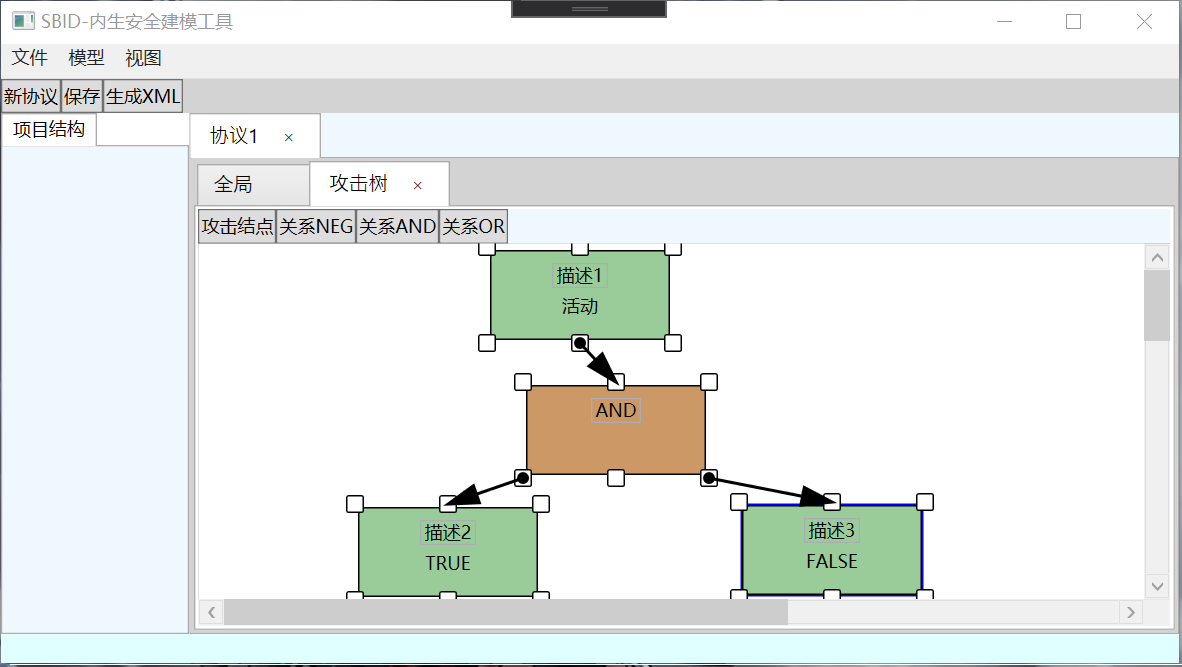
\includegraphics[width=12cm,height=6.75cm]{imgs/attack_tree_condition.png}
	\caption{设置结点状态}
	\label{attack_tree_condition}
\end{figure}

\par
右键点击活动状态的结点,点击计算,计算出该结点的状态。

\begin{figure}[h]
	\centering
	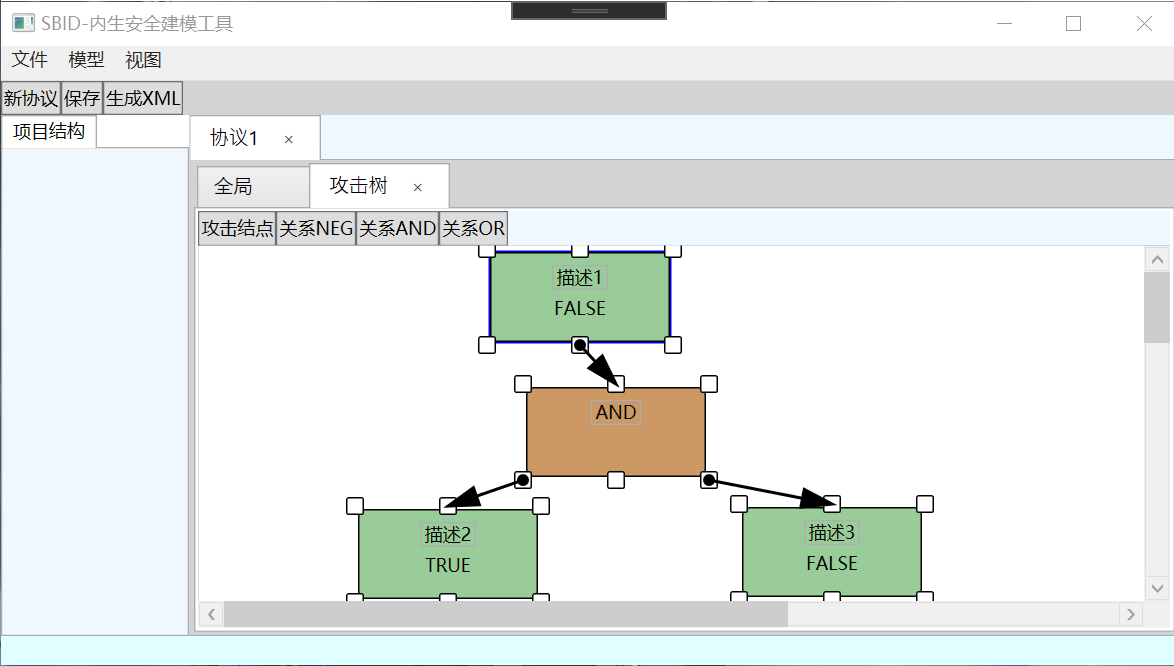
\includegraphics[width=12cm,height=6.75cm]{imgs/attack_tree_calculate.png}
	\caption{计算}
	\label{attack_tree_calculate}
\end{figure}